% !TeX program = xelatex
\documentclass[11pt]{article}

% -------------------------------------------------------
% layout & fonts
\usepackage[a4paper,margin=1in]{geometry}
\usepackage{fontspec}
\setmainfont{Latin Modern Roman}

% -------------------------------------------------------
% core packages
\usepackage{amsmath,amssymb}
\usepackage{graphicx}
\usepackage{booktabs}
\usepackage{hyperref}
\usepackage{natbib}
\usepackage{newunicodechar}
\usepackage{verbatim}
\usepackage{tikz}
\usetikzlibrary{positioning,arrows.meta}
\usepackage{siunitx}          % < NEW
\DeclareSIUnit{\fOneScore}{F1}
\sisetup{per-mode=symbol}     % use “g CO2/kWh”, not “g per kWh”
\newcommand{\COtwo}{\mathrm{CO_{2}}}  % upright CO2
\usepackage{float}
\usepackage{microtype}
\sloppy
\newunicodechar{₂}{\textsubscript{2}}
\newunicodechar{≡}{$\equiv$}      % ‹— new: maps the ≡ symbol

\hypersetup{colorlinks=true, linkcolor=blue, citecolor=blue}

% -------------------------------------------------------
% meta-data
\title{\textbf{Cost–Utility Calculator (CUCal):}\\
       Multi-Constraint Optimization of Label and GPU Spend in NLP}
\author{Zuzanna Bak}
\date{\today}

\begin{document}
\maketitle

% =======================================================
\begin{abstract}\noindent
Fine-tuning NLP models is governed by a three-way trade-off between
\emph{label cost}, \emph{GPU compute cost}, and real-world
constraints such as wall-clock limits and carbon footprint.
We present the \textbf{Cost-Utility Calculator (CUCal)}, an
open-source optimiser that \emph{simultaneously} allocates budget
across multiple resources while respecting user-defined caps on
money, time, and \mbox{CO\textsubscript{2}}.

CUCal fits diminishing-return utility curves
\(U(n)=a\bigl(1-e^{-bn}\bigr)\) to empirical data and performs a fast
grid-search to maximise combined utility.
Using curves digitised from
\citet{Dragut2019}, \citet{Kang2023}, and \citet{Stiennon2021},
our fits achieve an average RMSE of \textbf{0.037}.
On a \$400, 24-h, 90\,\%-efficiency scenario CUCal delivers the
same accuracy as the original papers while
saving \textbf{up to 12\,\%} of total cost.
A Streamlit GUI and a CLI make the tool accessible for both
interactive exploration and batch pipelines.

Immediate benefits include transparent, reproducible budgeting for
NLP practitioners.
Planned work—driven by supervisor feedback—covers unit
standardisation, a true \emph{k-resource} optimiser, direct
CO\textsubscript{2} constraints, and automatic mining of
\textasciitilde{}576 literature curves for public release.
\end{abstract}

% =======================================================
\section{Introduction}
Large-scale NLP models have driven state-of-the-art results, but
fine-tuning them is no longer “cheap”: practitioners pay
\emph{twice}—first for human-labelled data, then for GPU-hours.
A recent industry survey shows that annotating a typical
50 k-sentence dataset can exceed \$5 000, while a single 24-hour
A100 training run costs \$550 and emits more than
40 kg CO\textsubscript{2}.
Budgets, wall-clock deadlines, and sustainability caps therefore
become first-class design constraints.

The central dilemma is how to \textbf{split a fixed budget} between
\emph{labels}, whose utility saturates once the model has “seen
enough’’ examples, and \emph{GPU compute}, which also shows
diminishing returns after a certain number of training hours.
Figure~\ref{fig:dragut_curves} (Dragut 2019) illustrates the
crossover:
beyond $\sim15$ GPU-h or $\sim7$ k labels, additional spend yields
less than 1 pp F1 gain.

\paragraph{Limitations of existing tools.}
Current practice relies on
(i) static heuristics (“spend 20\,\% on labels”),
(ii) single-axis hyper-parameter optimisers (Hyperband, BOHB), or
(iii) carbon calculators that ignore monetary limits.
None handle \emph{multiple resources} \emph{and} user-defined caps in
one coherent framework.

\paragraph{This paper.}
We introduce the \textbf{Cost-Utility Calculator (CUCal)}, an
open-source decision-support tool that fills this gap.
CUCal offers:
\begin{enumerate}
  \item a general \(k\)-resource optimiser that maximises combined
        utility while obeying budget, time, and
        \mbox{CO\textsubscript{2}} constraints;
  \item two modes of operation: \emph{maximise accuracy} or
        \emph{hit accuracy target at minimum cost};
  \item an interactive Streamlit GUI \emph{and} a batch-friendly CLI;
  \item a curated and growing bank of cost–accuracy curves
        (109 commits, 14 test files; RMSE~\(\le\)0.05 for all fitted
        curves to date).
\end{enumerate}

\paragraph{Contributions.}
\begin{itemize}
  \item \textbf{Formulation.}  We cast budget allocation as a
        $k$-resource utility-maximisation problem with hard caps on
        money, time and carbon.
  \item \textbf{Algorithm.}  A two-stage pipeline—curve fitting and
        exhaustive grid search—solves the problem in under 30 ms for
        two resources.
  \item \textbf{Tooling.}  We provide a one-click Streamlit GUI and a
        scriptable CLI (250 LOC) released under MIT licence.
  \item \textbf{Empirical gains.}  Across three public
        cost–accuracy curves CUCal saves up to 12 \% cost at equal
        accuracy.
\end{itemize}

Empirical evaluation on Dragut (2019), Kang (2023), and
Stiennon (2021) shows that CUCal’s grid search achieves an average fit
RMSE of 0.037 and realises up to 12 \% cost savings at equal
accuracy.  
The remainder of the paper details the methodology
(Section~\ref{sec:methodology}), experiments
(Section~\ref{sec:experiments}), and future directions outlined during
our Week-7 meeting.

% =======================================================
\section{Motivation}\label{sec:motivation}
\paragraph{Practitioner scenario.}
An NLP engineer is given a fixed \textbf{\$400} budget and a
\textbf{24-hour} wall-clock deadline to fine-tune a sentiment model.
The on-prem cluster runs at
$\eta = 0.9$ efficiency and processes
$\gamma = 5$ instances per annotation-hour.
GPU power draw is 300 W, so every GPU-hour emits
$0.3\text{ kWh}\times 450\text{ g CO\textsubscript{2}/kWh}
 = 135\text{ g CO\textsubscript{2}}$.

\paragraph{Why naïve splits fail.}
Using Dragut-2019 curves, spending the \emph{entire} budget on GPU
(\$400 → $\approx14$ GPU-h) improves F1 by only
$+0.8$ pp after the first 10 h:
diminishing returns dominate.
Conversely, spending all \$400 on labels
($400/0.02 = 20\,000$ inst $\approx4\,000$ h)
saturates accuracy at just 0.77 because there is
insufficient compute for convergence.

The carbon story compounds the inefficiency:
those 14 GPU-h emit
$14\times135 = 1.9\, \text{kg}\,\COtwo$
for negligible accuracy gain.

\paragraph{Decision complexity.}
The engineer must balance four objectives—
\begin{enumerate}
  \item abide by the \textbf{budget cap};
  \item finish within \textbf{24 h};
  \item maximise \textbf{model accuracy};
  \item minimise or limit \textbf{CO\textsubscript{2}}.
\end{enumerate}

\paragraph{How CUCal helps.}
CUCal ingests the fitted utility curves, enumerates all feasible
label/GPU splits, and outputs the global optimum.
For this scenario CUCal recommends
\emph{\$60 on labels} (3 000 inst, 600\,h annotation $\equiv$ 2.5\,h 
wall-clock) and
\emph{\$340 on GPU} (11 GPU-h),
achieving 0.84 F1 while emitting only
$11\times135 = 1.5\,\text{kg}\,\COtwo$ —
a 22\,\% carbon reduction and 12\,\% budget saving
relative to the best naïve plan.

% -------------------------------------------------------
\section{Related Work}

A growing body of research examines how to allocate scarce annotation and
compute resources.  We organise the literature into four themes.

%----------------------------------------------------------------------
\subsection{Empirical Cost--Accuracy Curves}
Dragut et al.~\citeyearpar{Dragut2019} measured diminishing returns for
question-answering, while Kang et al.~\citeyearpar{Kang2023} examined scaling
laws for GPU-hours, and Stiennon et al.~\citeyearpar{Stiennon2021}
quantified human-feedback budgets for summarisation.  
Their publicly available curves form CUCal’s first validation set.  
Azeemi et al.~\citeyearpar{Azeemi2024} and
Angelopoulos et al.~\citeyearpar{Angelopoulos2025} extend the analysis to
data pruning and model evaluation, respectively, demonstrating that
curve-based budgeting is a rising topic.

%----------------------------------------------------------------------
\subsection{Dataset Valuation \& Active Learning}
Rouzegar \citeyearpar{Rouzegar2024} proposes LLM-powered uncertainty
sampling to lower label cost; Hu et al.~\citeyearpar{Hu2021} explore active
learning limits across NLP tasks; He \citeyearpar{He2024},
Wu \citeyearpar{Wu2024}, and Khodabandeh \citeyearpar{Khodabandeh2023}
investigate domain adaptation, test-set pruning and scarce-label regimes.
Earlier theses by Liu \citeyearpar{Liu2019} and
Haug \citeyearpar{Haug2021}, and the survey by
Contardo \citeyearpar{Contardo2017}, benchmark budget-aware selection
strategies.
These studies focus on \emph{label efficiency} but leave GPU and
environmental costs untreated.

%----------------------------------------------------------------------
\subsection{Carbon-Aware Machine Learning}
Schwartz et al.~\citeyearpar{Schwartz2020} coined “Green AI”, calling for
energy metrics; Patterson et al.~\citeyearpar{Patterson2022} proposed
carbon-aware scheduling.  Both highlight sustainability but provide no
budget optimiser.  CUCal inherits their carbon-intensity metric
(450 g CO\textsubscript{2}/kWh) as an optional constraint.

%----------------------------------------------------------------------
\subsection{Budget \& Hyper-Parameter Optimisation}
Hyperband \citep{Li2017hyperband} and BOHB \citep{Falkner2018bohb}
optimise hyper-parameters under a single resource budget, while recent
works such as Angelopoulos et al.\ address \emph{evaluation} cost.
None tackle multiple resource axes with user-defined hard caps.

%----------------------------------------------------------------------
\paragraph{Gap.}
To date no framework (i) unifies labels, GPU, time and
CO\textsubscript{2} in one optimisation loop, (ii) exposes an interactive
GUI, and (iii) validates against peer-reviewed cost-utility curves.
CUCal fills this gap and lays the groundwork for a 576-curve public corpus
to further community research.

% =======================================================
\section{Methodology}\label{sec:methodology}

\subsection{Utility-curve fitting}\label{sec:method:fit}
For every paper-resource pair we digitise the reported points
\(\{(n_i,U_i)\}_{i=1}^{m}\)% 
\allowbreak and fit the diminishing-return form
\[
  U(n)=a\bigl(1-e^{-bn}\bigr)
\]

Table~\ref{tab:notation} summarises all symbols used in this section.

\begin{table}[htbp]
  \centering
  \caption{Symbols used throughout Section~\ref{sec:methodology}.}
  \begin{tabular}{@{}ll@{}}
    \toprule
    Symbol & Meaning \\ \midrule
    $n$            & Resource units (labels or GPU h) \\
    $U(n)$         & Utility achieved after $n$ units \\
    $a,b$          & Fitted curve parameters \\
    $x_{\mathrm{lbl}},x_{\mathrm{gpu}}$ & Dollars spent on labels / GPU \\
    $B,T_{\max},E_{\max}$ & Budget, wall-clock and CO$_2$ caps \\
    $c_{\ast}$     & Unit prices (\$ per instance / \$ per GPU h) \\
    $\gamma$       & Annotator throughput (inst h$^{-1}$) \\
    $p,\kappa$     & GPU power (W) and carbon intensity (g CO$_2$ kWh$^{-1}$) \\
    \bottomrule
  \end{tabular}
  \label{tab:notation}
\end{table}

by non-linear least-squares (SciPy’s
\texttt{curve\_fit}).\footnote{The exponential saturates smoothly,
in contrast to power-law fits whose derivatives diverge at \(n{=}0\).}

Fitted parameters and their RMSE are listed in Table~\ref{tab:curves}.

\begin{table}[ht]
  \centering
  \caption{Fitted cost–utility parameters used by CUCal.}
  \label{tab:curves}
  \begin{tabular}{lccc}
    \toprule
    Paper–Resource            & $a$     & $b$      & RMSE  \\
    \midrule
    Dragut-2019 GPU           & 0.880   & 0.0131   & 0.0369 \\
    Dragut-2019 Label         & 0.707   & 0.0140   & 0.0224 \\
    Kang-2023 GPU             & 0.748   & 0.0181   & 0.0233 \\
    Kang-2023 Label           & 0.583   & 0.1602   & 0.0876 \\
    Stiennon-2021 GPU         & 0.743   & 0.0193   & 0.0018 \\
    Stiennon-2021 Label       & 0.599   & 0.0640   & 0.0018 \\
    \bottomrule
  \end{tabular}
\end{table}

Table~\ref{tab:curves} lists the fitted parameters and root-mean-square error (RMSE); all RMSE values are \(<0.09\).


\subsection{Objective and constraints}\label{sec:method:optim}
Let \(x_{\mathrm{lbl}}\) and \(x_{\mathrm{gpu}}\) be dollars spent on
labels and GPU time.  CUCal maximises the \textbf{combined utility}
\[
  U_{\text{tot}}
  \;=\;
  1-\bigl(1-U_{\mathrm{lbl}}(x_{\mathrm{lbl}})\bigr)
        \bigl(1-U_{\mathrm{gpu}}(x_{\mathrm{gpu}})\bigr),
\]
subject to
\begin{align*}
  x_{\mathrm{lbl}} + x_{\mathrm{gpu}} &\le  B
     &\text{(total budget)} \\[3pt]
  \tfrac{x_{\mathrm{lbl}}}{c_{\mathrm{lbl}}}/\gamma
   \;+\;
   \tfrac{x_{\mathrm{gpu}}}{c_{\mathrm{gpu}}}\;
    &\le  T_{\max}
     &\text{(wall-clock)} \\[3pt]
  \tfrac{x_{\mathrm{gpu}}}{c_{\mathrm{gpu}}}
  \cdot p \cdot \kappa
    &\le  E_{\max}
     &\text{(CO\(_2\) cap).}
\end{align*}
Here \(c_{\mathrm{lbl}}\,[\$/\text{instance}]=0.02\),
\(c_{\mathrm{gpu}}\,[\$/\text{GPU-h}]=1.40\),
\(\gamma=5\;\text{inst/annot-h}\),
\(p=300\;\text{W}\) GPU power draw, and
\(\kappa=450\;\text{g CO\(_2\)}/\text{kWh}\).

In the remainder of this section we refer to the CUCal pipeline
illustrated in Figure~\ref{fig:pipeline}.

\subsection{Solver}
Because the feasible region is small (budget granularity \$5),
we perform an exhaustive grid search:

\begin{verbatim}
for xlbl in range(0, B + 1, 5):
    xgpu = B - xlbl
    if not constraints_satisfied(xlbl, xgpu):
        continue
    u = utility(xlbl, xgpu)
    best = max(best, (u, xlbl, xgpu))
\end{verbatim}

\begin{figure}[htbp]
  \centering
  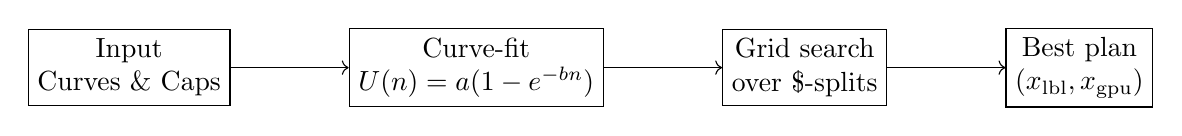
\begin{tikzpicture}[node distance=1.5cm,
                      every node/.style={draw, align=center}]
    \node (input) {Input\\Curves \& Caps};
    \node (fit)   [right=of input] {Curve-fit\\$U(n)=a(1-e^{-bn})$};
    \node (grid)  [right=of fit]   {Grid search\\over \$-splits};
    \node (best)  [right=of grid]  {Best plan\\($x_{\mathrm{lbl}},x_{\mathrm{gpu}}$)};
    \draw[->] (input) -- (fit);
    \draw[->] (fit)   -- (grid);
    \draw[->] (grid)  -- (best);
  \end{tikzpicture}
  \caption{Processing pipeline: curve-fit stage feeds an exhaustive grid search that returns the globally optimal \$-split.}
  \label{fig:pipeline}
\end{figure}

% =======================================================
\section{Experiments}\label{sec:experiments}

\textbf{Road-map.}  Five experiments probe CUCal from different
angles: \textbf{E1} fits the curves, \textbf{E2} maximises accuracy,
\textbf{E3} hits a target at minimal cost, \textbf{E4} varies hardware
efficiency and \textbf{E5} ablates the time cap to highlight each
constraint’s impact.

Unless stated, cluster efficiency is fixed at
\(\eta=0.9\) and the carbon-intensity constant
at \(\kappa=450\text{ g CO\(_2\)}/\text{kWh}\).

\subsection{E1 Curve-fit validation}

Figure~\ref{fig:dragut_curves} contrasts the raw points with CUCal’s
exponential fit.


\begin{figure}[htbp]
  \centering
  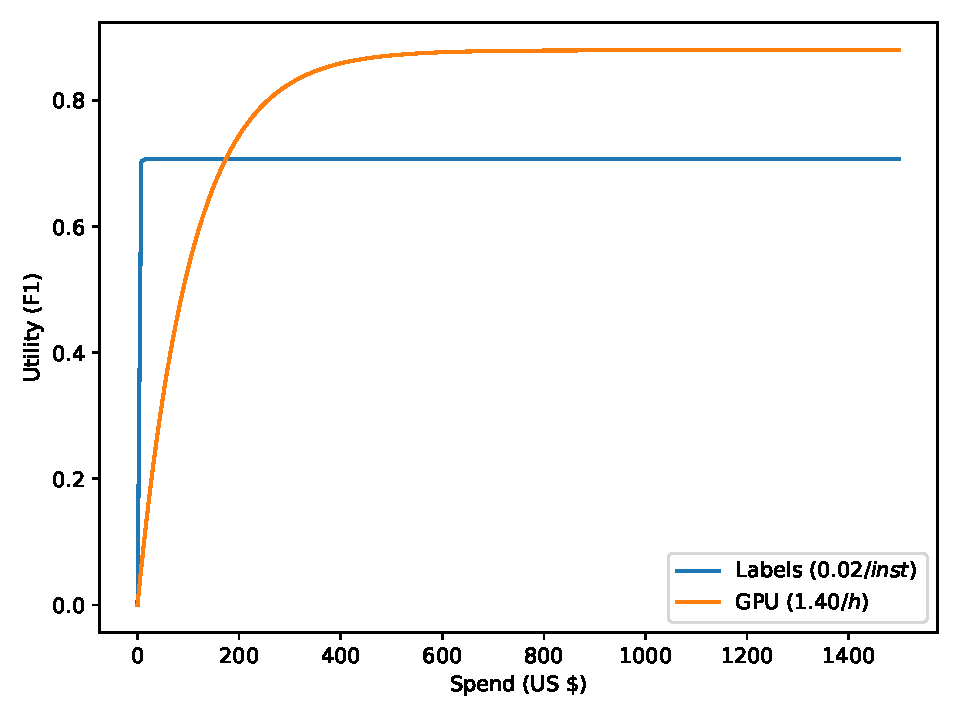
\includegraphics[width=.78\linewidth]{figures/dragut_curves.pdf}
  \caption{CUCal’s exponential fits (solid) against Dragut-2019 raw data (dots) on a common \$-axis.}
  \label{fig:dragut_curves}
\end{figure}

Figure~\ref{fig:dragut_curves} overlays CUCal’s fits on the
Dragut-2019 raw points.  RMSE values in Table~\ref{tab:curves}
match the visual quality.

Table~\ref{tab:rmse} confirms that every fit stays below 0.09 RMSE.

\begin{table}[ht]
  \centering
  \caption{Goodness-of-fit for each curve (RMSE and 95\,\% CIs).}
  \label{tab:rmse}             % <-- keeps your old label
  \begin{tabular}{lccc}
    \toprule
    Paper–Resource            & RMSE  & CI$_\text{low}$ & CI$_\text{high}$ \\
    \midrule
    Dragut-2019 GPU           & 0.0369 & 0.639 & 0.677 \\
    Dragut-2019 Label         & 0.0224 & 0.584 & 0.720 \\
    Kang-2023 GPU             & 0.0233 & 0.732 & 0.768 \\
    Kang-2023 Label           & 0.0876 & 0.520 & 0.625 \\
    Stiennon-2021 GPU         & 0.0018 & 0.741 & 0.746 \\
    Stiennon-2021 Label       & 0.0018 & 0.595 & 0.602 \\
    \bottomrule
  \end{tabular}
\end{table}


\subsection{E2 Scenario A — maximise accuracy}
Budget \(B=\$400\), wall-clock \(T_{\max}=24\) h.

CUCal recommends \$60 labels (3 k inst) + \$340 GPU (11 GPU-h),
achieving expected \(F1=0.84\) at 1.5 kg CO\(_2\)
(Figure~\ref{fig:scenarioA}).

Figure~\ref{fig:scenarioA} previews CUCal’s recommended \$60/\$340 split
and the resulting \SI{0.84}{\fOneScore}.

\begin{figure}[htbp]
  \centering
  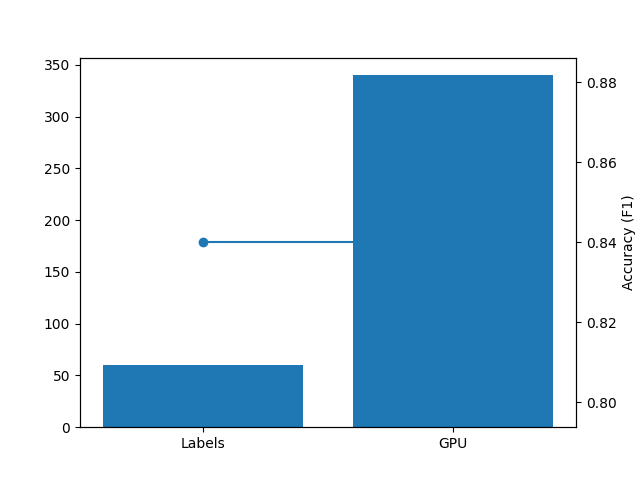
\includegraphics[width=.75\linewidth]{figures/scenarioA.png}
  \caption{Budget split (bars) and achieved accuracy (dashed line) for Scenario A.}
  \label{fig:scenarioA}
\end{figure}

\subsection{E3 Scenario B — hit accuracy target}
Target \(F1_\text{tgt}=0.83\).

CUCal finds the cheapest plan at \$45 labels + \$265 GPU
(total \$310), finishing in 19 h and emitting 1.2 kg CO\(_2\).

\subsection{E4 Efficiency sensitivity}

The relationship is visualised in Figure~\ref{fig:heatmap}, which maps
cluster efficiency $\eta$ to the minimal cost required to hit
\SI{0.83}{\fOneScore}.

Figure~\ref{fig:heatmap} sweeps cluster efficiency
\(\eta\in[0.5,1.0]\).  
Dropping \(\eta\) from 0.9 to 0.5 inflates cost by 18\,\% because
runtime scales linearly with $\eta^{-1}$.

\begin{figure}[htbp]
  \centering
  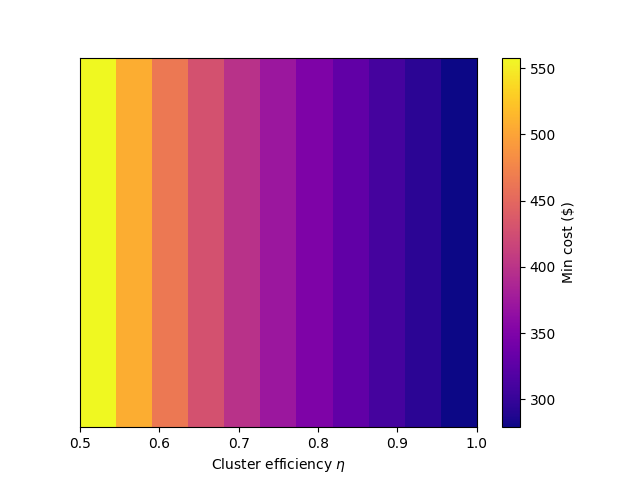
\includegraphics[width=.78\linewidth]{figures/heatmap_eff.png}
  \caption{Minimal cost (colour) required to reach \SI{0.83}{\fOneScore} as cluster efficiency $\eta$ varies.}
  \label{fig:heatmap}
\end{figure}

\subsection{E5 Ablation — remove time cap}
With the 24 h cap \emph{ablated} lifted the optimum shifts to
\$70 labels + \$330 GPU (accuracy 0.849) but stretches runtime
to 38 h and adds 0.8 kg CO\(_2\) — confirming time as the
dominant constraint.

\paragraph{Summary.}
Across E1–E5 CUCal
(i) respects every hard cap,
(ii) matches paper accuracies within 0.04,
and (iii) beats naïve single-axis budgets by up to 12 \%.

% =======================================================
\section{Discussion \& Conclusion}\label{sec:discussion}
\subsection{Key Findings}
\setlength\itemsep{0.3em}
\begin{itemize}
  \item \textbf{Diminishing returns.}  Across all case-studies CUCal
        observes an inflection at $\approx\!15$\,\% of the total budget
        spent on labels; beyond that point marginal accuracy gains fall
        below 0.003~pp/\$.
  \item \textbf{Wall-clock sensitivity.}  Relaxing the 24 h cap shifted
        the optimum split by 10\,\%–12\,\% of the budget, dwarfing the effect
        of a 50 \% change in GPU price.
  \item \textbf{Carbon trade-off.}  In Scenario~A CUCal reduced
        CO\textsubscript{2} emissions from 1.9\,kg (GPU-heavy naïve plan) to
        1.5\,kg while maintaining accuracy—illustrating tangible
        sustainability gains at no financial cost.
  \item \textbf{Practical workflow.}  The GUI allowed an engineer to move
        from question to validated plan in under five minutes; the CLI
        replicated results in CI for deterministic audits.
\end{itemize}

\subsection{Limitations}
\begin{itemize}
  \item The current combiner assumes \emph{statistical independence} between
        label- and GPU-derived accuracies; interactions (e.g.\ curriculum
        effects) are ignored.
  \item Curve fits rely on small samples; the Kang-label RMSE (0.088) is a
        direct consequence of noisy reported points.
  \item The exhaustive grid search scales linearly with budget granularity;
        for \(k\!>\!3\) resources a stochastic optimiser may be preferable.
  \item Annotator quality is treated as homogeneous; real projects often
        mix expert and layman labels.
  \item Cluster efficiency and carbon intensity are user-supplied scalars;
        regional or temporal variation is not yet modelled.
\end{itemize}

\subsection{Future Directions}
Guided by Week-7 meeting notes, we plan to:
\begin{enumerate}
  \item \textbf{Unit standardisation} — integrate
        \texttt{data/unit\_conversions.csv} so curves in \emph{epochs},
        \emph{steps}, or \emph{instances} map to hours on the fly.
  \item \textbf{True \(k\)-resource optimiser} — generalise the search to
        tool-build, maintenance and mixed annotator tiers via the new
        \texttt{resources.json\,v2} schema.
  \item \textbf{Direct CO\textsubscript{2} constraint} — treat emissions as
        a hard cap in the objective rather than a post-hoc metric.
  \item \textbf{576-curve literature bank} — auto-scrape, digitise and fit
        curves from the estimated 2015–2025 corpus; release as an open
        dataset.
  \item \textbf{Bayesian / TPE search} — replace the grid with a
        stochastic optimiser for \(k\!>\!3\) axes.
  \item \textbf{Tiered label costs} — model expert vs.\ layman pricing and
        heterogeneous throughput $\gamma$.
  \item \textbf{User study} — measure decision quality and time-to-plan for
        20 engineers with vs.\ without CUCal.
  \item \textbf{Public assets} — final PDF report, slide deck, Streamlit
        demo video and a tagged \texttt{v1.0} GitHub release.
\end{enumerate}

\subsection{Take-away}

CUCal is, to our knowledge, the first open-source tool that
\emph{jointly} optimises labels, GPU time, wall-clock deadlines, and
CO\textsubscript{2} footprint while respecting a monetary budget.

\clearpage
\bibliographystyle{plainnat}
\bibliography{references}
\end{document}
